% !TeX spellcheck = en_GB
\documentclass[../summary.tex]{subfiles}

\begin{document}
	\section{Human behaviour}
	
		\subsection{Study guide}
			A lot of the discussed global challenges and their solutions require a lot of change in behaviour from us humans. This however, is not easy. Because of this it's important to understand how the human brain works, what drives us and what motivates us. \\
			\\
			We will first explore the way in which we make decisions when faced with different dilemma's or situations. Once we know more about this, we can take a look at how to change these thoughts and convince people. Finally, we will take a look at how biasses affect our thinking. 
		\subsection{Conditioning vs. motivating}
			\textbf{Edward Thorndyke} was one of the most important psychology researchers to live. He started his career at Harvard studying ``the instinctive and intelligent behaviour of chickens''. Moving on to the study of cats at Columbia University. In his experiments with cats, he deprived them of food and let them solve some sort of puzzle to get access to food. When he would repeat this sequence with the same cats, he noticed they would very quickly catch on to the solution, and by the third repetition, they could solve the puzzle in a matter of seconds. \\
			\\
			Similar and systematic experiments gave way to the \textbf{law of effect}: `responses that produce a satisfying effect in a particular situation become more likely to occur again in that situation, and responses that produce a discomforting effect become less likely to occur again in that situation'.\\
			\\
			Later on this law was studied by \textbf{Boris Frederick Skinner}.   He discovered the animals which were most likely to have good learning results with rewards: rats, mice, pigeons and pigs. He also pioneered a way to prove learned behaviour by systematically withholding reward. \\
			\\
			The act of learning and unlearning was central in psychology research for many decades. Thousands of papers were written about the effectiveness of rewarding because it was a good motivator in the tested animal groups. 
			\subsubsection{Motivation}
				When it comes to \textbf{rewarding behaviour}, a complication is that people overestimate the importance of \textbf{extrinsic motives} in the behaviour of others, while they look at their own behaviour as more \textbf{intinsically motivated}.\\
				\\
				A study by Chip Heath illustrated this by asking people to rank the order of importance of eight motives in their professional life. The first four were extrinsic: pay, benefits, praise and security; the four others were intrinsic: learning, developing, skills and feeling good with worthwhile work. On average, the first four out of five were intrinsic motivators, pay was only ranked on the fourth place. \\
				\\
				When the participants were asked to do this for their peers, pay moved up to the second place. Going even further, when they were asked to do this for their managers or bank clerks, they ranked pay on place one. Those same managers and bank clerks only ranked pay on position seven for themselves. \\
				\\
				Because of these insights, most psychologists think of rewards and sometimes punishment to aid behavioural change in people. But getting people intrinsically motivated for change is more qualitative and at least as important as the reward structure. 
		\newpage
		\subsection{Social dilemmas}
			Psychologists use certain experiments as \textbf{a paradigm to study social dilemma's}. An example of this is a game where there are a green card and a blue card. You and seven others need to choose a colour without knowing what the others will do. Choosing the green card yields you five euros, if you pick the blue card you get 24 euros, but everyone gets a penalty of 3 euros. \\
			\\
			This game has parallels to the consumption of meat and climate change. If everyone would eat less meat, it would have a huge impact. But is an individual person willing to let go of this steak for this goal? Many other situations follow this train of thought, like watering your lawn so it looks good during a drought. Picking the blue card while everyone else picks green is advantageous to one self, choosing green would make the whole group better of. \\
			\\
			These types of paradigms are all derived from the \textbf{prisoner dilemma}: imagine that two people, A and B, commit a crime. The authorities know this but don't have the proper evidence. They get interrogated and given the choice to confess or not to confess without knowing what their respective partners will do. The outcome of their decision is  depicted in figure \ref{fig:12-prisoners-dilemma}. \\
			
			\begin{figure}[h]
				\centering
				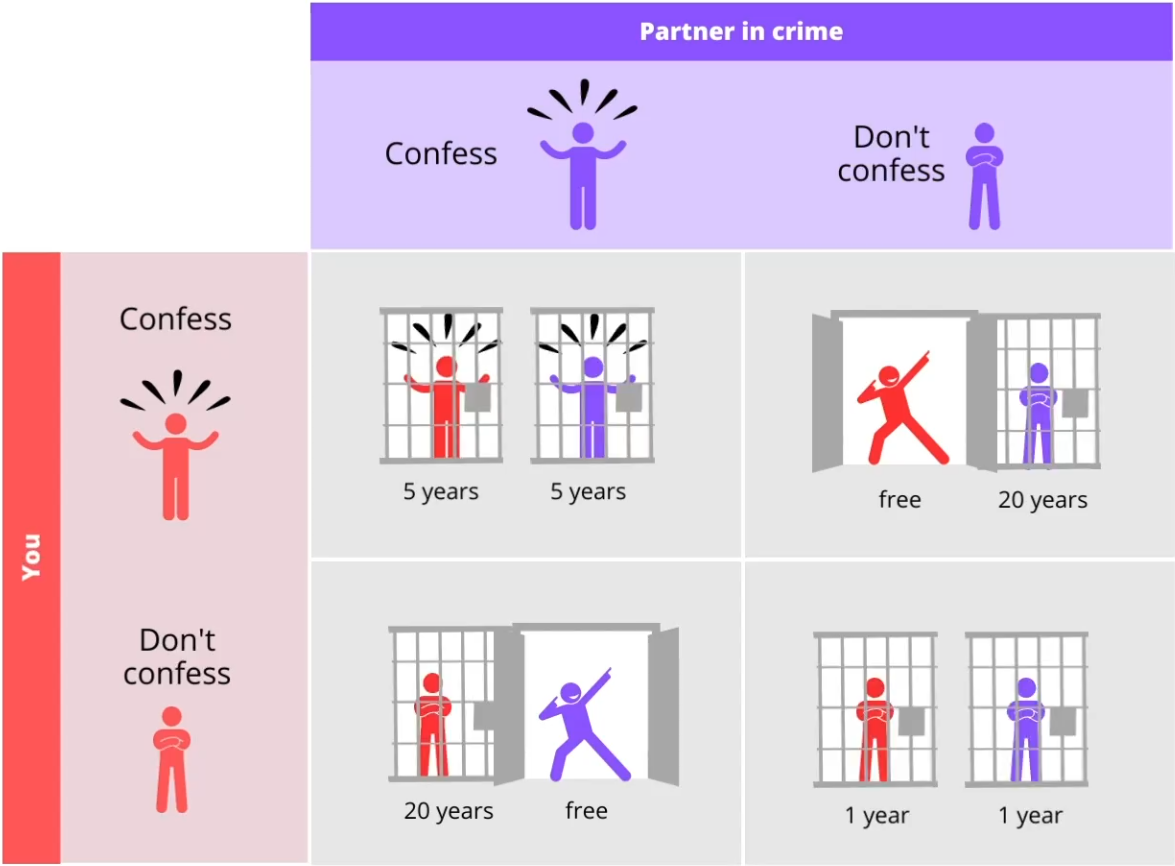
\includegraphics[width=0.7\linewidth]{../images/12-prisoners-dilemma.png}
				\caption{depictions of the outcomes for the prisoner dilemma}
				\label{fig:12-prisoners-dilemma}
			\end{figure}
			What must one do when faced with this situation? It really depends on what your partner does. But in general it is better to confess, this minimizes the chance of you going to prison for a long time. On the other hand, not confessing would lead to the minimal amount of jail time between them. \\
			\\
			In the prisoner dilemma, the participants are not anonymous, they each bare a large responsibility towards the outcome of the situation. When talking about climate change and meat consumption, this is not the case. There are many parties involved which makes it completely different. \\
			\\
			\newpage
			Going back to the card experiment we can now find some meaning in a social dilemma. Going with the green card is called a \textbf{cooperative choice}, while the blue pick would be called a \textbf{competitive choice}.  A number of factors have been experimentally shown to have an effect on the results:
			\begin{enumerate}
				\item It is important that people thoroughly realize the mutual dependence in the situation. This grows when consecutive choices have to be made with feedback about the results after every choice. Awareness of the impact one has is very important. 
				\item The number of parties involved in the dilemma affects cooperation. The more participants, the more competitive choices will be made. This is because people try to ride free on the cooperative choices others make. 
				\item Communication promotes cooperation. 
				\item Cooperation decreases when the choices are made by groups instead of individuals. This is because a sort of `us' vs `them' mentality crops up. 
				\item Competition decreases when individual choices are more visible. This is because nobody wants to be perceived as the bad guy who ruins it for the rest.
				\item Research points to important individual differences amongs types of participants
			\end{enumerate}
		\newpage
		\subsection{Individual differences}
		
		\subsection{Thoughtful or automatic}
		
		\subsection{Persuasive communication}
		
		\subsection{Stakeholder system}
		
		\subsection{Biases}
		
		\subsection{Questions and feedback}
\end{document}